\documentclass[journal]{IEEEtran}
\usepackage{amsmath,amssymb}
\usepackage{graphicx}
\usepackage{booktabs}
\usepackage{array}
\usepackage{url}
\usepackage{cite}
\usepackage[hidelinks]{hyperref}
% Generated by scripts/paper_numbers.py from committed results; do not edit by hand.
% Anchor check passed: confirmatory macros identical from verdict.json and endpoints.csv.
\newcommand{\ACobstViolPct}{89}
\newcommand{\ACrrViolPct}{85}
\newcommand{\AciHione}{\ensuremath{-4.85}}
\newcommand{\AciHithree}{\ensuremath{-43.04}}
\newcommand{\AciHitwo}{\ensuremath{-14.98}}
\newcommand{\AciLoone}{\ensuremath{-5.78}}
\newcommand{\AciLothree}{\ensuremath{-45.11}}
\newcommand{\AciLotwo}{\ensuremath{-16.49}}
\newcommand{\Adiffone}{\ensuremath{-5.30}}
\newcommand{\Adiffthree}{\ensuremath{-44.08}}
\newcommand{\Adifftwo}{\ensuremath{-15.72}}
\newcommand{\AfirstObstPeriod}{30}
\newcommand{\AfiveCount}{1}
\newcommand{\AfiveGap}{0.087}
\newcommand{\AfiveH}{\ensuremath{-0.00777}}
\newcommand{\AhoNegPct}{80}
\newcommand{\AlphaStar}{10}
\newcommand{\Apassone}{met}
\newcommand{\Apassthree}{met}
\newcommand{\Apasstwo}{met}
\newcommand{\Apone}{\ensuremath{2.6\times 10^{-144}}}
\newcommand{\Apthree}{\ensuremath{<10^{-300}}}
\newcommand{\Aptwo}{\ensuremath{<10^{-300}}}
\newcommand{\AucPooled}{0.96}
\newcommand{\Aupperone}{\ensuremath{-4.82}}
\newcommand{\Aupperthree}{\ensuremath{-42.95}}
\newcommand{\Auppertwo}{\ensuremath{-14.92}}
\newcommand{\BCobstViolPct}{4}
\newcommand{\BCrrViolPct}{36}
\newcommand{\BciHione}{5.27}
\newcommand{\BciHithree}{11.27}
\newcommand{\BciHitwo}{10.53}
\newcommand{\BciLoone}{4.35}
\newcommand{\BciLothree}{9.84}
\newcommand{\BciLotwo}{9.10}
\newcommand{\Blossone}{4.81}
\newcommand{\Blossthree}{10.56}
\newcommand{\Blosstwo}{9.81}
\newcommand{\Bpassone}{not met}
\newcommand{\Bpassthree}{not met}
\newcommand{\Bpasstwo}{not met}
\newcommand{\Bupperone}{5.31}
\newcommand{\Bupperthree}{11.33}
\newcommand{\Buppertwo}{10.59}
\newcommand{\CapBindMax}{8}
\newcommand{\CapBindMin}{1}
\newcommand{\CapMedMax}{0.78}
\newcommand{\CapMedMin}{0.72}
\newcommand{\CciHione}{0.0126}
\newcommand{\CciHithree}{0.0290}
\newcommand{\CciHitwo}{0.0212}
\newcommand{\CciLoone}{0.0108}
\newcommand{\CciLothree}{0.0266}
\newcommand{\CciLotwo}{0.0192}
\newcommand{\Celigone}{9{,}000}
\newcommand{\Celigthree}{9{,}000}
\newcommand{\Celigtwo}{9{,}000}
\newcommand{\Cexclone}{0}
\newcommand{\Cexclthree}{0}
\newcommand{\Cexcltwo}{0}
\newcommand{\Cincone}{0.0117}
\newcommand{\Cincthree}{0.0278}
\newcommand{\Cinctwo}{0.0202}
\newcommand{\Cnormone}{0.0126}
\newcommand{\Cnormthree}{0.0291}
\newcommand{\Cnormtwo}{0.0213}
\newcommand{\CollBmone}{0}
\newcommand{\CollBmthree}{0}
\newcommand{\CollBmtwo}{0}
\newcommand{\CollOffone}{483}
\newcommand{\CollOffthree}{4{,}319}
\newcommand{\CollOfftwo}{1{,}490}
\newcommand{\CollOnone}{0}
\newcommand{\CollOnthree}{0}
\newcommand{\CollOntwo}{0}
\newcommand{\Cpassone}{not met}
\newcommand{\Cpassthree}{not met}
\newcommand{\Cpasstwo}{not met}
\newcommand{\Cupperone}{0.0127}
\newcommand{\Cupperthree}{0.0291}
\newcommand{\Cuppertwo}{0.0213}
\newcommand{\FailOffone}{5.4}
\newcommand{\FailOffthree}{48.0}
\newcommand{\FailOfftwo}{16.6}
\newcommand{\FailOnone}{0.1}
\newcommand{\FailOnthree}{3.9}
\newcommand{\FailOntwo}{0.8}
\newcommand{\GapAmedCm}{3.3}
\newcommand{\GapBmedCm}{14.4}
\newcommand{\GoalBmone}{48.8}
\newcommand{\GoalBmthree}{19.3}
\newcommand{\GoalBmtwo}{53.5}
\newcommand{\GoalOffone}{54.7}
\newcommand{\GoalOffthree}{32.0}
\newcommand{\GoalOfftwo}{66.6}
\newcommand{\GoalOnone}{49.9}
\newcommand{\GoalOnthree}{21.5}
\newcommand{\GoalOntwo}{56.8}
\newcommand{\GroupA}{2{,}274}
\newcommand{\GroupAnb}{15}
\newcommand{\GroupAobst}{2{,}259}
\newcommand{\GroupAprime}{2{,}540}
\newcommand{\GroupB}{11{,}255}
\newcommand{\InfBmone}{0}
\newcommand{\InfBmthree}{0}
\newcommand{\InfBmtwo}{0}
\newcommand{\InfHdiffMax}{\ensuremath{4.3\times 10^{-8}}}
\newcommand{\InfNear}{410}
\newcommand{\InfOnone}{6}
\newcommand{\InfOnthree}{352}
\newcommand{\InfOntwo}{75}
\newcommand{\InfRepro}{433}
\newcommand{\InfRobots}{433}
\newcommand{\InfSlackMax}{\ensuremath{-8.4\times 10^{-9}}}
\newcommand{\InfSlackMin}{\ensuremath{-4.9\times 10^{-6}}}
\newcommand{\InfTotal}{433}
\newcommand{\OnBmGoalMax}{3.2}
\newcommand{\OnBmGoalMin}{1.0}
\newcommand{\OnMinusBmGoalone}{1.0}
\newcommand{\OnMinusBmGoalthree}{2.2}
\newcommand{\OnMinusBmGoaltwo}{3.2}
\newcommand{\PairsPerDensity}{9{,}000}
\newcommand{\RgrOffone}{94.6}
\newcommand{\RgrOffthree}{51.3}
\newcommand{\RgrOfftwo}{83.2}
\newcommand{\RgrOnone}{87.1}
\newcommand{\RgrOnthree}{35.0}
\newcommand{\RgrOntwo}{69.5}
\newcommand{\SelGoalfive}{1{,}936}
\newcommand{\SelGoalhalf}{0}
\newcommand{\SelGoalone}{255}
\newcommand{\SelGoalten}{2{,}224}
\newcommand{\SelGoaltwo}{1{,}184}
\newcommand{\SelInffive}{61}
\newcommand{\SelInfhalf}{1{,}251}
\newcommand{\SelInfone}{4}
\newcommand{\SelInften}{129}
\newcommand{\SelInftwo}{11}
\newcommand{\SelN}{5{,}400}
\newcommand{\TObmone}{51.2}
\newcommand{\TObmthree}{80.7}
\newcommand{\TObmtwo}{46.5}
\newcommand{\TOfi}{9{,}211}
\newcommand{\TOfiObst}{9{,}143}
\newcommand{\TOfiOffColl}{5{,}699}
\newcommand{\TOfiOffGoal}{2{,}274}
\newcommand{\TOfiPct}{61}
\newcommand{\TOng}{5{,}670}
\newcommand{\TOngOffTO}{5{,}362}
\newcommand{\TOngPct}{38}
\newcommand{\TOoffone}{39.9}
\newcommand{\TOoffthree}{20.0}
\newcommand{\TOofftwo}{16.9}
\newcommand{\TOonTotal}{15{,}038}
\newcommand{\TOonone}{50.1}
\newcommand{\TOonthree}{74.6}
\newcommand{\TOontwo}{42.4}
\newcommand{\ThrMatchObstFive}{43.1}
\newcommand{\ThrOffGoal}{51.1}
\newcommand{\ThrOnGoal}{42.7}
\newcommand{\ThrRetObstFive}{84.4}
\newcommand{\TrialsTotal}{27{,}000}
\newcommand{\Verdictone}{not shown useful}
\newcommand{\Verdictthree}{not shown useful}
\newcommand{\Verdicttwo}{not shown useful}
\newcommand{\Vp}{0.50}

\hyphenation{MAPPO VMAS Newcombe}

\begin{document}
\title{An Execution-Time CBF-QP Safety Filter on Frozen MAPPO Formation Policies:
A Pre-Specified Paired Evaluation in Simulation}

\author{Al~Mahdi~Sallam%
\thanks{A.~M.~Sallam is with the Department of Electrical Engineering, King Fahd University of
Petroleum and Minerals (KFUPM), Dhahran, Saudi Arabia (e-mail: mahdisallam860@gmail.com).}%
\thanks{DRAFT, not for distribution; authorship and framing pending advisor review.}}

\markboth{Draft, not for distribution}%
{Sallam: Execution-Time CBF-QP Safety Filter on Frozen MAPPO Formation Policies}

\maketitle

\begin{abstract}
We evaluate whether one execution-time, decentralised control-barrier-function quadratic-programme
(CBF-QP) safety filter, placed between frozen multi-agent PPO (MAPPO) formation policies and a
simulated team of three unicycle-modelled robots, meets non-inferiority criteria that the author fixed
before the test. Nine frozen actors (three training runs, three checkpoints each), which had not met
the study's filter-off competence gate (pooled over 2, 5 and 8 obstacles), were evaluated on reserved, previously unused layouts with
one, two and three obstacles (\PairsPerDensity{} paired trials per obstacle count) with the filter off,
the filter on at $\alpha^\star=\AlphaStar$\,s$^{-1}$ (the largest gain the sampled-data condition
admits, selected on validation layouts), and a brake applied on the same constraints. The filter
reduced the share of trials ending in collision or QP infeasibility at every obstacle count (from
\FailOffone\% to \FailOnone\%, \FailOfftwo\% to \FailOntwo\% and \FailOffthree\% to \FailOnthree\%),
while the share not reaching the goal rose (from \NonGoalOffone\% to \NonGoalOnone\%,
\NonGoalOfftwo\% to \NonGoalOntwo\% and \NonGoalOffthree\% to \NonGoalOnthree\%). Under the pre-set
criteria it was \emph{not shown useful} at any obstacle count: non-inferiority was not established for
goal completion (margin 5 percentage points; at one obstacle the estimated loss, \Blossone{} points, was
inside the margin but its upper bound was not) or for formation error over the common executed prefix
(margin 0.01\,m). The brake had no collisions, cannot be infeasible by construction, and reached the
goal \OnBmGoalMin--\OnBmGoalMax{} points less often than the filter. Exploratory, post hoc analyses of
the saved logs show that most lost completions ended as timeouts during which the filter was overriding
the policy's command, and that every infeasible QP occurred with a constraint at its stand-off, where
stopping is only marginally inadmissible. Claims cover this filter instantiation and these nine actors
in one simulated scenario.
\end{abstract}

\begin{IEEEkeywords}
Control barrier functions, safety filter, multi-agent reinforcement learning, MAPPO, formation
control, sampled-data systems, pre-specified evaluation.
\end{IEEEkeywords}

\section{Introduction}
\IEEEPARstart{R}{einforcement-learning} policies for multi-robot formations are commonly trained without safety
constraints \cite{brunke2022}, and a control-barrier-function (CBF) safety filter \cite{ames2019}
can be added at execution time without retraining. Whether such a filter is \emph{useful}, here: reduces
collision-or-infeasible outcomes without a loss of goal completion or formation quality larger than
margins fixed in advance, is an empirical question for a given policy family. This draft reports a pre-specified paired evaluation
of one such filter, a decentralised sampled-data CBF-QP, on frozen MAPPO \cite{yu2022mappo} actors
in a VMAS \cite{bettini2022vmas} differential-drive formation-navigation scenario, followed by clearly
labelled exploratory analyses of where, among the paired trials, the lost completions occurred.

\paragraph{Contributions.} Studies of safe multi-agent learning mostly add safety during training or
learn it together with the policy. Among those that act at execution, one evaluates with and without
its filter a policy that was trained with the filter, one compares the unfiltered policy mainly
qualitatively with a centralised filter on double integrators, and one adds a learned correction to a
frozen policy without stating that its comparison is paired (Section~\ref{sec:related},
Table~\ref{tab:related}). This draft adds:
(i) a paired evaluation, with criteria and margins fixed before the test and reserved test layouts,
of a decentralised execution-time CBF-QP filter on a family of nine frozen MAPPO actors that never saw
the filter, together with a brake comparator on the same layouts;
(ii) a confirmatory result for these actors: collision-or-infeasible outcomes fell at every density,
but non-inferiority in goal completion and formation error was not established, with outcomes,
failure types and per-seed variation reported in full;
(iii) exploratory, clearly labelled analyses of where the lost completions occurred (timeouts during
which the filter overrode the policy's command, on layouts where the unfiltered runs passed close to
obstacles) and of the infeasible states (each with a constraint at its stand-off); and
(iv) the code, saved per-step logs of every final-test trial and scripts that regenerate every number,
so the analyses can be repeated without re-running trials.

\paragraph{Research question.} Does this execution-time CBF-QP filter, applied to frozen MAPPO
formation policies trained without it, reduce collisions, and at what cost in formation error,
goal completion and deadlock?

\paragraph{Motivating hypotheses.} The study was motivated by three hypotheses stated
in the study's earlier research proposal, quoted here: ``H1: collisions fall. H2: formation error and
completion time rise, more so in denser layouts. H3: most failures under filtering come from
deadlock or infeasible steps rather than slower progress.'' The proposal defined deadlock as ``centroid
progress below a set distance over a set window''; the protocol's stalled flag implements this as a
TIMEOUT whose centroid-to-goal distance fell by less than 0.05\,m over the last 50 executed periods. The
flag measures progress toward the goal, not distance travelled or stationarity: a team moving sideways,
circling or moving away also satisfies it. These hypotheses
motivate the design; they do not extend the locked confirmatory claims, which are the three
criteria of Section~\ref{sec:design}. Section~\ref{sec:discussion} maps each hypothesis to the
evidence and states which evidence is confirmatory and which is exploratory.

\section{Related work}\label{sec:related}
Safe learning in robotics is surveyed in \cite{brunke2022} and control barrier functions in
\cite{ames2019}. Multi-agent approaches differ in when safety enters. Some apply a CBF shield during
training \cite{cai2021} or learn barrier certificates together with the policy
\cite{qin2021,zhang2025gcbf,zhang2025dgppo}; some filter during both training and execution
\cite{choi2025,dawood2025}; one learns a safety correction on top of a frozen MAPPO policy
\cite{deng2026}; and one filters at execution a separately obtained RL planner, using a centralised
QP for double-integrator agents \cite{vinod2022}. Table~\ref{tab:related} summarises them. Here
\emph{paired on/off} means that the same frozen policy is evaluated with and without the filter on
matched layouts; a comparison between separately trained policies (a training ablation) does not count
as paired in this sense. \cite{dawood2025} does report a paired test in this sense, but for a policy
trained with its filter, which is then deactivated; the present study evaluates policies that never
saw the filter. The classifications were checked against the papers on 26 October 2026: against the
full text for \cite{cai2021,choi2025,dawood2025,deng2026,vinod2022} and against the abstract only
for \cite{qin2021,zhang2025gcbf,zhang2025dgppo}, where ``not reported in abstract'' marks what could
not be checked.

Sampled-data CBF formulations that account for inter-sample behaviour are studied in
\cite{singletary2020,breeden2022,tan_zocbf,liu_sacbf}; the margin used here is of the
input-independent kind, a bound over the whole input set that does not depend on the applied command.
CBF-QP filters can introduce undesirable stable equilibria \cite{reis2021}. Decentralised equal-split
(``half-responsibility'') constraints go back to \cite{wang2017,vandenberg2011}, and stopping as a
feasibility-preserving backup is used in \cite{chen2021}. The offset (barrier) point for unicycles
is used in \cite{emam2019}. Hidden assumptions in CBF safety claims are discussed in
\cite{kim2026}. Input-dependent inter-sample bounds used for trigger timing appear in
\cite{yang2019}. Interval estimates and per-seed reporting for RL evaluation are argued for in
\cite{agarwal2021}.

\begin{table*}[t]
\centering\footnotesize
\caption{Related multi-agent studies. ``Paired on/off'' = the same frozen policy evaluated with and
without the filter on matched layouts. Checked against the full text (F) or the abstract only (A) on
26 October 2026.}
\label{tab:related}
\footnotesize
\begin{tabular}{>{\raggedright\arraybackslash}p{2.2cm}>{\raggedright\arraybackslash}p{4.8cm}>{\raggedright\arraybackslash}p{4.0cm}>{\raggedright\arraybackslash}p{4.0cm}c}
\toprule
Study & When safety enters & Paired on/off & Outcomes reported & Checked\\
\midrule
Cai et al. \cite{cai2021} & CBF shield during training (also claimed for deployment) & No: separately trained agents & collisions, training reward & F\\
Qin et al. \cite{qin2021} & certificates learned with the policy; test-time refinement & not reported in abstract & safety, task completion & A\\
GCBF+ \cite{zhang2025gcbf} & graph CBF and distributed policy learned together & not reported in abstract & safety, goal reaching & A\\
DGPPO \cite{zhang2025dgppo} & graph CBF learned simultaneously with the policy & not reported in abstract & task performance, safety rate & A\\
Choi et al. \cite{choi2025} & CBVF filter in the second half of training and at execution & No: separately trained variants & goal reach, near collisions, conflicts, travel time & F\\
Deng et al. \cite{deng2026} & learned correction added to a frozen MAPPO policy & base policy reported; pairing not stated & return, arrival rate, violation rate & F\\
Dawood et al. \cite{dawood2025} & MPC filter in training and execution & Yes, for a policy trained with the filter & goals, timeouts, collisions, time, formation error & F\\
Vinod et al. \cite{vinod2022} & centralised QP filter at execution on a separately obtained RL planner (filter use in training not stated) & same policy and start states, reported mainly qualitatively & completion, deadlock, loitering & F\\
This study & decentralised CBF-QP at execution; policies trained without it & Yes: 9{,}000 matched layouts per density & collisions, infeasibility, completion, formation, stalls & --\\
\bottomrule
\end{tabular}
\end{table*}

\section{System and filter}\label{sec:system}
\paragraph{Robots and task.} Three differential-drive robots, modelled as unicycles with a box
constraint on $(v,\omega)$ (wheel-speed coupling is not modelled), with axle-centre pose $(x,y,\theta)$,
body disc of radius $R=0.10$\,m, and command $u=(v,\omega)$ in the box
$\mathcal U=\{-0.5\le v\le 0.5\ \mathrm{m/s},\ |\omega|\le 1\ \mathrm{rad/s}\}$ follow the unicycle model
\begin{equation}
\dot x = v\cos\theta,\qquad \dot y = v\sin\theta,\qquad \dot\theta=\omega ,
\end{equation}
with commands held over each control period $\Delta=0.1$\,s (zero-order hold). The team moves a
triangular formation (slot radius 0.30\,m) through a field of $K$ circular obstacles of radius
$R_o=0.20$\,m to a goal within a horizon of 400 periods. A \emph{layout} fixes the obstacle centres and the
initial poses: the team starts on its triangle slots around the centroid $(-1.5,0)$\,m (position noise
0.03\,m, heading noise 0.15\,rad) and must bring its centroid to $(1.5,0)$\,m; the $K$ obstacle centres
are drawn uniformly in $[-0.8,0.8]\times[-0.9,0.9]$\,m with surface gaps of at least 0.10\,m and clear of
the start and goal; there are no walls. The \emph{density} $K$ is the number of obstacles in this fixed
field. GOAL is reached at the first post-step state with the centroid within 0.10\,m of the goal and the
formation error $e(t)$ of Section~\ref{sec:design} at most 0.10\,m; COLLISION (robot--obstacle or
robot--robot overlap) is scored on the swept path and ends the trial; an infeasible QP ends the trial as
INFEASIBLE at that period, before the period's motion; otherwise the trial ends as TIMEOUT.

\paragraph{Offset point and barriers.} The filter constrains the point
$p=(x+\ell\cos\theta,\ y+\ell\sin\theta)$, $\ell=0.05$\,m, for which
\begin{equation}
\dot p = J(\theta)\,u,\quad J(\theta)=\begin{bmatrix}\cos\theta & -\ell\sin\theta\\ \sin\theta & \ell\cos\theta\end{bmatrix},\quad \det J=\ell ,
\end{equation}
so every barrier below has relative degree one in $(v,\omega)$. For an obstacle with centre $c$
and robots $i\ne j$ the barriers are
\begin{equation}
\begin{aligned}
h_o&=\|p-c\|^2-D_o^2, & D_o&=R+\ell+R_o,\\
h_{ij}&=\|p_i-p_j\|^2-D_{rr}^2, & D_{rr}&=2(R+\ell).
\end{aligned}
\end{equation}
Because $\|x-p\|=\ell$, the body disc lies inside the \emph{cover disc} of radius $R+\ell$ around
$p$, so $h\ge0$ implies that the body discs do not overlap ($h>0$: strictly separated), for every
heading. The converse does not hold: heading straight at an obstacle, a robot has $h_o<0$ at any body
clearance below $2\ell=\TwoEllCm$\,cm (Fig.~\ref{fig:f0}).

\begin{figure}[t]\centering
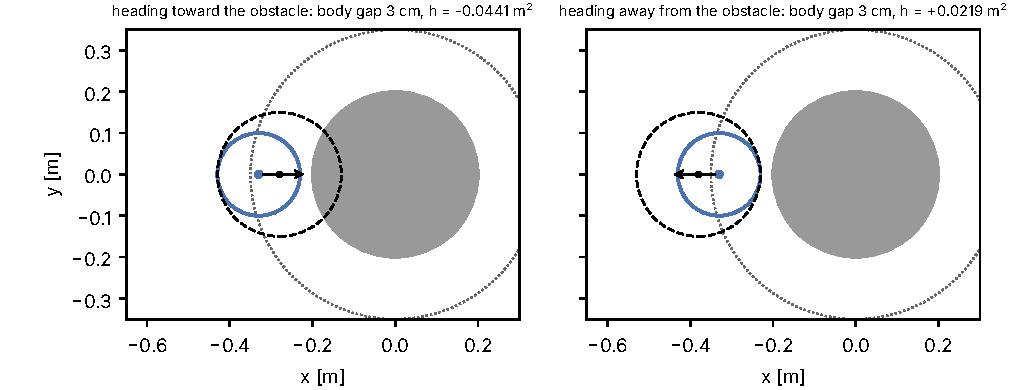
\includegraphics[width=\columnwidth]{../figures/F0_cover_disc_schematic.pdf}
\caption{Analytic schematic (no data). Body disc (solid), axle centre, offset point $p$ and cover disc
of radius $R+\ell$ (dashed) next to an obstacle (grey) whose barrier boundary $\|p-c\|=D_o$ is dotted. With
the same 3\,cm body clearance, the cover barrier is negative when the robot heads toward the obstacle and
positive when it heads away.}\label{fig:f0}
\end{figure}

\paragraph{Sampled-data condition.} The implemented filter uses the following lemma with a
two-sided bound on $\ddot h$; only the lower bound is needed.

\emph{Lemma 1 (one-sided form).} Let $u$ be held on $[t_k,t_k+\Delta]$, $\ddot h\ge -M$ on that
interval with $M\ge0$, $\alpha\Delta\le 1$ and $h(t_k)\ge 0$. If
$\dot h(t_k)+\alpha h(t_k)\ge \delta=M\Delta/2$, then
$h(t_k+s)\ge (1-\alpha s)\,h(t_k)\ge 0$ for all $s\in[0,\Delta]$.

This is the second-order approach of \cite{breeden2022} (Theorem~3, stated there with the opposite
sign convention for $h$; $\gamma\le1$ corresponds to $\alpha\Delta\le1$). With
$\bar v=\max|v|=0.5$\,m/s, $\bar\omega=\max|\omega|=1$\,rad/s,
$V_p=\sqrt{\bar v^2+\ell^2\bar\omega^2}\approx0.5025$\,m/s (an upper bound on $\|\dot p\|$) and $A_p=\bar\omega V_p$ (an upper bound on $\|\ddot p\|$ under a held command), the implemented margins use the
two-sided bounds of the design document,
\begin{equation}
\begin{aligned}
\delta_o(d)&=\tfrac{\Delta}{2}\big[2V_p^2+2(d+V_p\Delta)A_p\big],\\
\delta_{ij}(d)&=\tfrac{\Delta}{2}\big[8V_p^2+4(d+2V_p\Delta)A_p\big],
\end{aligned}
\end{equation}
where $d$ is the barrier-point distance at $t_k$: $d=\|p-c\|$ for an obstacle row and
$d=\|p_i-p_j\|$ for a pair row. These bounds follow from $\|\ddot p\|\le A_p$ under a held command,
$\ddot h_o=2\|\dot p\|^2+2(p-c)^\top\ddot p$ and $\|p(t)-c\|\le d+V_p\Delta$ within the period (pair
rows: relative speed and acceleration at most $2V_p$ and $2A_p$). Only the lower bound $\ddot h\ge-M$
is needed, so the $2V_p^2$ and $8V_p^2$ terms add conservatism. At $\alpha\Delta=1$ the lemma still gives
$h\ge0$ over the whole period, but no strictly positive endpoint bound.

\paragraph{Equal split and the per-robot QP.} With $g_o=2J(\theta_i)^\top(p_i-c)$ and
$g_{ij}=2J(\theta_i)^\top(p_i-p_j)$, robot $i$ solves at every period
\begin{equation}
\begin{aligned}
\min_{u\in\mathcal U}\ & \tfrac12\|u-u_{\rm nom}\|^2\\
\text{s.t. }& g_o^\top u\ \ge -\alpha h_o+\delta_o(d),\\
& g_{ij}^\top u\ \ge -\tfrac{\alpha}{2}h_{ij}+\tfrac12\delta_{ij}(d),
\end{aligned}
\end{equation}
with one obstacle row for every obstacle whose barrier-point distance is $d\le 1.0$\,m and one
neighbour row for every neighbour with $d\le 1.5$\,m, where $u_{\rm nom}$ is the frozen actor's deterministic command. The sensing ranges exceed
$D_o+V_p\Delta$ and $D_{rr}+2V_p\Delta$ (both about 0.40\,m), so an omitted barrier cannot reach zero
within the period; within range the filter uses exact obstacle centres and exact, undelayed neighbour
poses. Each robot takes half of every pair condition (equal split); the two halves sum to the pair
condition of Lemma~1 when both robots compute their rows from the same state, apply their commands over
the same period and both QPs are feasible. In this simulation the first two hold by construction (every
robot reads the exact, synchronous joint state), so ``decentralised'' refers to how the computation is
split; with inconsistent or delayed states no guarantee is claimed.

\emph{Stand-off.} Because $\delta>0$, the zero command satisfies an obstacle row only if
$h_o\ge h^\star:=\delta_o(d)/\alpha$, and a pair row only if $h_{ij}\ge\delta_{ij}(d)/\alpha$. We call
$h^\star$ the \emph{stand-off}: the smallest barrier value at which a robot may stop. At $\alpha^\star$
and $d=D_o$ the obstacle stand-off lies \StandOffObstCm\,cm of barrier-point distance beyond $D_o$, so a
stopped robot needs a body clearance from an obstacle between about \CoverBandLoCm\,cm (heading away)
and \CoverBandHiCm\,cm (heading toward it).

\emph{Guarantee and assumptions.} By induction over periods, Lemma~1 and the equal split keep every
barrier non-negative for all $t$, so the bodies never overlap, under these assumptions: (A1) the
realised motion is the exact unicycle arc of the held command; (A2) exact, noise-free states and obstacle
positions; (A3) synchronous, undelayed neighbour states within range; (A4) zero-order hold over $\Delta$,
with the QP solved within the period; (A5) $h\ge0$ for every barrier at the start; (A6) static circular
obstacles and no walls; (A7) the command box contains $u=0$ and is shared by the policy clip and the
QP; (A8) $\alpha\Delta\le1$, $\ell>0$ and the range rule above; (A9) every QP is feasible. A trial whose
QP becomes infeasible violates A9 and ends as INFEASIBLE. In simulation A1 holds to the integrator's
float32 accuracy. The two-variable QP is solved by enumerating its candidate optima (the unconstrained optimum, the
projection onto each constraint line and every pairwise vertex) and keeping the closest feasible one;
this is implemented in floating-point arithmetic with a feasibility tolerance of $10^{-9}$ on
normalised rows; the QP is INFEASIBLE when no candidate satisfies every enabled row within this
tolerance. There is no fallback, so an infeasible QP ends the trial. A period is an \emph{intervention}
when $\|u-\mathrm{clip}(u_{\rm nom})\|_\infty>10^{-6}$.
The B-match comparator (a brake matched to the filter's rows) applies $(0,\bar\omega_{\rm nom})$, with
$\bar\omega_{\rm nom}$ the clipped nominal turn rate, whenever the clipped nominal command violates one
of these rows at the same gain. It solves no QP, so it cannot be INFEASIBLE by construction. With $v=0$
the body disc does not move, so a braked robot cannot strike a static obstacle during that period, but
B-match carries no barrier-level guarantee ($p$ rotates, so $h$ can decrease) and none against a moving
neighbour.

\section{Policy and training}\label{sec:policy}
\paragraph{Observation and reward.} Each robot observes, in its body frame: its slot error relative
to the centroid, the centroid-to-goal vector (norm-clipped at 2.0\,m), teammates' relative positions
and headings, the eight nearest obstacles within 2.0\,m (relative centre, surface gap, present flag)
and an agent one-hot. The per-period reward is
$10\cdot$(centroid progress toward the goal) $-1\cdot$(mean slot error) $-0.01\cdot$(control effort)
$-10\cdot$[collision] $-0.2\cdot\sum_{\rm pairs}\max(0,1-\text{clearance}/0.15\,\mathrm{m})$, summed over robot--obstacle and robot--robot pairs (surface clearance); control effort is the mean over robots of $(v/0.5)^2+\omega^2$; a collision
ends the episode and a timeout is bootstrapped. The filter is never used in training.

\paragraph{MAPPO and curriculum.} A compact PyTorch implementation of MAPPO \cite{yu2022mappo} (shared Gaussian actor with tanh-bounded
mean, centralised critic, GAE with $\gamma=0.99$, $\lambda=0.95$, clip 0.2, 10 epochs, 16 minibatches,
learning rates $3\times10^{-4}$ actor and $10^{-3}$ critic, no entropy bonus, gradient-norm clip 0.5,
hidden layers $128\times128$ (actor) and $256\times256$ (critic), initial action standard deviation half
of each half-range, 384 parallel environments of 64 steps) was
trained with three seeds through a curriculum $K=0\to1\to2\to3\to(2,5,8)$ with maximum stage budgets of 1, 2,
4, 4 and 8 million environment steps; a stage ended early once the GOAL rate on the validation layouts (Section~\ref{sec:design})
reached 80\% at every stage density, which happened in the $K=0$ and $K=1$ stages for all three seeds.
The final stage trains on $K=2,5,8$ only; $K=1$ and $K=3$ are absent from it but were encountered
in earlier stages. The implementation was sanity-checked only on the stock VMAS
navigation task, where the deterministic policy reached \MappoNavSuccess\% success on 200 fixed
episodes (uniform random: \MappoNavRandom\%).

\paragraph{Checkpoints and gate history.} The nine actors are the early, middle and late checkpoints
of the final curriculum stage of each seed, fixed by an iteration rule (first saved checkpoint with
$r\ge\lceil n/3\rceil$, $r\ge\lceil 2n/3\rceil$, and $r=n$, where $r$ is the iteration counted within the
final stage and $n=326$ is its length). The three checkpoints of one seed come from the same training
run and are not independent policies.
Seed~1 crashed at global iteration 565 (a layout-sampler stall) and was resumed from the state it had
saved at iteration 546: actor, critic, optimiser states, value normaliser and action-sampling
generator were restored bit for bit, but the environments, the position in the training-layout chunk
and the global random-number state were not, and iterations 547--565 (466{,}944 environment steps) were
discarded. Actors s1\_middle and s1\_late come from the resumed run; s1\_early predates the crash
(audit/PROVENANCE.md, Section~3). The global random-number state is used neither for action sampling
nor for layouts. The resumed actors cannot be regenerated by re-running seed~1; the committed checkpoint
files (SHA-256 in \texttt{results/phase1/checkpoint\_selection.json}) are the reference. The
filter-off competence gate fixed before training (pooled GOAL $\ge$ 50\% over $K=2,5,8$; below it the
policy ``rarely reaches the goal'') was not met by any checkpoint: the best pooled GOAL rate was
\GateVoneBest\% for a first configuration (four observed obstacles, no proximity penalty, no
curriculum) and \GateVtwoBest\% after the observation, reward, PPO settings and curriculum were revised
(the configuration described above). $K=5,8$ were therefore moved to stress cells and $K=1,2,3$ became
the primary densities, chosen after the actors' filter-off validation results had been seen so that both
completions and collisions occur. The results therefore concern a weak, collision-prone policy family;
they do not predict the filter's cost on policies that keep more clearance.
Table~\ref{tab:baseline} shows the filter-off baseline of the nine actors on validation layouts.

\begin{table}[t]
\centering\small
\caption{Filter-off baseline on validation layouts (200 per cell): GOAL / COLLISION / TIMEOUT (\%) per actor and
obstacle count $K$ (descriptive context; $K=4$ was an intermediate diagnostic).}
\label{tab:baseline}
\resizebox{\columnwidth}{!}{%
\begin{tabular}{lcccccc}
\toprule
actor & $K=1$ & $K=2$ & $K=3$ & $K=4$ & $K=5$ & $K=8$\\
\midrule
\TabBaselineRows
\bottomrule
\end{tabular}}
\end{table}

\section{Experimental design}\label{sec:design}
The protocol was locked by the author before any filter-on data with the frozen MAPPO actors
existed; the margins and decisions were chosen without advisor review
(Section~\ref{sec:disclosures}). Filter-on results did exist before the lock in two other forms:
engineering stress tests of the filter with random and adversarial stand-in controllers
(\EngStressTrials{} paired trials) and paired demonstration runs with an obstacle-blind stand-in
controller. Neither used the frozen MAPPO actors. The frozen-MAPPO development sweep on validation
layouts followed the lock, and the reserved final evaluation followed the gain selection.
\emph{Validation layouts} (200 per $K$, seed $2{,}000{,}000+K$) were used to advance curriculum stages,
for the filter-off gate and Table~\ref{tab:baseline}, and for gain selection. \emph{Final-test layouts}
(1{,}000 per actor and $K$) were not used before the final test.

The gain was selected on existing validation layouts from $\alpha\in\{0.5,1,2,5,10\}$\,s$^{-1}$ by the
highest pooled filter-on GOAL count over the nine actors and $K=1,2,3$ (ties: fewer INFEASIBLE, then the
larger gain). The final test used 1{,}000 reserved layouts per actor and density, each run with the
filter off, the filter on at $\alpha^\star$ and B-match at $\alpha^\star$. Usefulness at a density
required all of: (a) a one-sided exact McNemar reduction in COLLISION-or-INFEASIBLE; (b) GOAL loss
(off minus on) with one-sided 98.33\% upper bound at most 0.05; (c) the equal-actor-weighted mean
increase in formation error over the common executed prefix with stratified bootstrap 98.33\% upper
bound at most 0.01\,m. Within a density the three criteria form an intersection--union test, so no
split across (a)--(c) is needed; each is tested one-sided at $0.05/3$, a Bonferroni split over the three
density claims, so the familywise error over the three usefulness claims is at most 0.05. Criterion (a)
is decided by the exact McNemar test (its interval bound is reported); (b) is decided by the interval
bound. For (a) and (b) the paired difference in proportions has a two-sided 96.67\% Newcombe score
interval \cite{newcombe1998} (Wilson score limits combined through the estimated correlation
$\hat\phi$), whose appropriate limit gives the one-sided 98.33\% bound. The locked protocol labels this
interval ``method~10'' but describes it as combining the Wilson limits through $\hat\phi$ ``without
continuity correction'', which is Newcombe's method~8; the analysis code, committed before any
frozen-MAPPO filter-on data, implements that description. Method~10 applies a continuity correction to
$\hat\phi$. The label inconsistency was found after the final test.
Recomputing every bound for (a) and (b) with method~10 changes it by less than 0.001
percentage points and changes no criterion (\texttt{scripts/newcombe\_method10\_check.py}); the
reported numbers are those of the locked code. The margins are the author's judgement, fixed
without advisor review or external calibration; for any other margin, the 98.33\% bounds in
Table~\ref{tab:conf} give the smallest margin each criterion would have met. Per-seed and per-actor results, episode length,
reached-goal-region (centroid within 0.30\,m of the goal before any collision or infeasibility),
final centroid-to-goal distance, TIMEOUT and the stalled flag were pre-declared as secondary and
descriptive.

\paragraph{Formation endpoint (criterion (c)).} For a trial, let $T$ be the number of control
periods actually executed: a period that ends in COLLISION counts, while an attempted period that an
infeasible QP prevented does not. Let $x_r(t)$ be robot $r$'s position at the post-step state after
period $t$, $\bar x(t)$ the team centroid and $s_r$ its slot offset; the formation error is
\begin{equation}
e(t)=\tfrac13\textstyle\sum_{r=1}^{3}\big\|x_r(t)-\bar x(t)-s_r\big\|,\qquad t=1,\dots,T,
\end{equation}
so the initial state and the frozen samples after termination are excluded. For pair $i$ with
executed counts $T_{\rm off}$ and $T_{\rm on}$, the common executed prefix has length
$L_i=\min(T_{\rm off},T_{\rm on})$ and, for $L_i>0$,
\begin{equation}
\Delta e_i=\frac1{L_i}\sum_{t=1}^{L_i}\big[e_{\rm on}(t)-e_{\rm off}(t)\big].
\end{equation}
For pairs with $L_i=0$ (an arm infeasible at its first period) the formation difference is undefined;
they are excluded from (c) and never counted as zero. Each arm keeps its recorded outcome in (a) and
(b): an infeasible arm counts as a failure and as not reaching GOAL, the other arm keeps its own
outcome, and no pair is assigned a GOAL loss by the exclusion. With $\mathcal E_p$
the eligible pairs of actor $p$, the estimand is the equal-actor mean
\begin{equation}
\overline{\Delta e}=\frac19\sum_{p=1}^{9}\frac1{|\mathcal E_p|}\sum_{i\in\mathcal E_p} \Delta e_i .
\end{equation}
Its upper bound is a stratified paired percentile bootstrap: pairs are resampled with replacement
within each actor, $\overline{\Delta e}$ is recomputed with the same equal weights, $B=\BootReps$ replicates are
drawn with \texttt{numpy.random.default\_rng(\BootSeed)}, and the bound is the $1-0.05/3$ quantile of
the replicates (\texttt{numpy.quantile}, method \texttt{linear}). A normal bound from the per-actor
variances is reported as a cross-check. If any actor has fewer than \MinEligible{} eligible pairs,
criterion (c) is inconclusive and the weights are not renormalised. In the final test every pair was
eligible (Table~\ref{tab:conf}). The common prefix had median length \LMedone, \LMedtwo{} and
\LMedthree{} periods at $K=1,2,3$ (quartiles \LQloone--\LQhione, \LQlotwo--\LQhitwo{} and
\LQlothree--\LQhithree), so (c) mainly reflects early transit; when the unfiltered run collides, the
prefix ends at that collision and excludes the filter's later avoidance manoeuvre.

\section{Results}\label{sec:results}
\paragraph{Gain selection (development data).} Pooled filter-on GOAL counts over \SelN{} validation
trials were \SelGoalhalf, \SelGoalone, \SelGoaltwo, \SelGoalfive{} and \SelGoalten{} for
$\alpha=0.5,1,2,5,10$, with \SelInfhalf, \SelInfone, \SelInftwo, \SelInffive{} and \SelInften{}
INFEASIBLE outcomes, so $\alpha^\star=\AlphaStar$ (Fig.~\ref{fig:f1}). GOAL rose with every step up
the grid, and $\alpha^\star$ is also the largest gain with $\alpha\Delta\le1$: the evaluated filter is
the least conservative admissible member of this family on the development data.

\begin{table*}[t]
\centering\footnotesize
\caption{Confirmatory results, filter on ($\alpha^\star=\AlphaStar$) versus filter off, nine actors
pooled, \PairsPerDensity{} pairs per density. Differences in percentage points (pp); one-sided bounds
at 98.33\%; 95\% intervals descriptive.}
\label{tab:conf}
\begin{tabular}{lccc}
\toprule
 & $K=1$ & $K=2$ & $K=3$\\
\midrule
COLLISION-or-INFEASIBLE, off $\to$ on (\%) & \FailOffone{} $\to$ \FailOnone & \FailOfftwo{} $\to$ \FailOntwo & \FailOffthree{} $\to$ \FailOnthree\\
(a) difference on$-$off [pp] & \Adiffone & \Adifftwo & \Adiffthree\\
\quad 98.33\% upper; 95\% CI & \Aupperone; [\AciLoone, \AciHione] & \Auppertwo; [\AciLotwo, \AciHitwo] & \Aupperthree; [\AciLothree, \AciHithree]\\
\quad one-sided exact $p$; criterion & \Apone; \Apassone & \Aptwo; \Apasstwo & \Apthree; \Apassthree\\
GOAL off / on (\%) & \GoalOffone{} / \GoalOnone & \GoalOfftwo{} / \GoalOntwo & \GoalOffthree{} / \GoalOnthree\\
(b) GOAL loss off$-$on [pp] & \Blossone & \Blosstwo & \Blossthree\\
\quad 98.33\% upper (margin 5); criterion & \Bupperone; \Bpassone & \Buppertwo; \Bpasstwo & \Bupperthree; \Bpassthree\\
(c) formation increase [m] & \Cincone & \Cinctwo & \Cincthree\\
\quad bootstrap 98.33\% upper (margin 0.01) & \Cupperone & \Cuppertwo & \Cupperthree\\
\quad normal cross-check; eligible / excluded & \Cnormone; \Celigone / \Cexclone & \Cnormtwo; \Celigtwo / \Cexcltwo & \Cnormthree; \Celigthree / \Cexclthree\\
\quad criterion & \Cpassone & \Cpasstwo & \Cpassthree\\
\midrule
Verdict & \Verdictone & \Verdicttwo & \Verdictthree\\
\bottomrule
\end{tabular}
\end{table*}

\paragraph{Confirmatory results.} Table~\ref{tab:conf} gives the confirmatory results. Criterion (a)
was met at every density; (b) and (c) were met at none, so the filter was \emph{not shown useful under
the pre-set criteria} at $K=1,2,3$. At $K=1$ the GOAL-loss estimate (\Blossone{} pp) lies inside the
5\,pp margin and only its upper bound (\Bupperone{} pp) exceeds it; at $K=2,3$ the estimates exceed the
margin. Read together, the filter changed collision-or-infeasible outcomes by \Adiffone, \Adifftwo{}
and \Adiffthree{} pp and lost \Blossone, \Blosstwo{} and \Blossthree{} pp of GOAL; how these trade off
depends on the relative cost of a collision and a timeout in an application, and the margins encode one
such judgement. With the filter on there were \CollOnone, \CollOntwo{} and
\CollOnthree{} collisions and \InfOnone, \InfOntwo{} and \InfOnthree{} INFEASIBLE trials;
TIMEOUT rose from \TOoffone\%, \TOofftwo\% and \TOoffthree\% to \TOonone\%, \TOontwo\% and
\TOonthree\% (Fig.~\ref{fig:f2}). B-match had \CollBmone, \CollBmtwo{} and \CollBmthree{} collisions
and \InfBmone, \InfBmtwo{} and \InfBmthree{} INFEASIBLE outcomes, and reached GOAL in \GoalBmone\%,
\GoalBmtwo\% and \GoalBmthree\% of trials; the filter reached GOAL \OnMinusBmGoalone,
\OnMinusBmGoaltwo{} and \OnMinusBmGoalthree{} percentage points more often (descriptive). B-match
solves no QP, so its zero INFEASIBLE count holds by construction.

\paragraph{Filter on versus B-match (pre-declared secondary, descriptive).} The locked protocol
pre-declared a comparison of the filter with B-match at $\alpha^\star$ on the same pairs and
endpoints, with intervals, and states that nothing confirmatory follows from it.
Table~\ref{tab:onbm} gives the paired differences, always filter on minus B-match, on all
\PairsPerDensity{} pairs per density. The intervals are two-sided 95\% Newcombe method~10
intervals: Wilson score limits for each arm, combined through the continuity-corrected correlation
$\hat\phi$, whose numerator $ad-bc$ is replaced by $\max(ad-bc-n/2,0)$ when $ad-bc>0$ ($a$: event
in both arms, $b$: filter on only, $c$: B-match only, $d$: neither). They were computed with a new
implementation after the method~8/method~10 discrepancy described in Section~\ref{sec:design} was
found; the historical confirmatory intervals and \texttt{cbf\_study/stats.py} are unchanged.
B-match had no COLLISION or INFEASIBLE outcome, so for that endpoint one marginal variance is zero,
the correlation is undefined, and $\hat\phi=0$ is used. The formation row is the equal-actor mean
over pairs of $\frac{1}{L}\sum_{t=1}^{L}[e_{\text{on}}(t)-e_{\text{B-match}}(t)]$, with
$L=\min(T_{\text{on}},T_{\text{B-match}})$ and $e(t)$ recomputed from the saved poses, with a 95\%
stratified paired percentile bootstrap within actor (the locked settings: \BootReps{} resamples,
seed \BootSeed); \OnBmFormExclone, \OnBmFormExcltwo{} and \OnBmFormExclthree{} pairs had $L=0$
and were excluded. The filter reached GOAL more often than B-match and timed out less often at every
density, and had more COLLISION-or-INFEASIBLE outcomes; B-match cannot be infeasible by construction,
so that row compares the filter's infeasible terminations with none. No test or verdict is
attached to these differences.

\begin{table*}[t]
\centering\footnotesize
\caption{Filter on versus B-match at $\alpha^\star$ (pre-declared secondary, descriptive; nothing
confirmatory follows). Paired differences, filter on minus B-match, on all \PairsPerDensity{} pairs per
density: percentage points with two-sided 95\% Newcombe method-10 intervals; formation: equal-actor
mean common-prefix difference in metres with a 95\% stratified paired bootstrap interval. B-match
cannot be INFEASIBLE by construction.}
\label{tab:onbm}
\begin{tabular}{lccc}
\toprule
 & $K=1$ & $K=2$ & $K=3$\\
\midrule
GOAL [pp] & \OnBmGoalDiffone & \OnBmGoalDifftwo & \OnBmGoalDiffthree\\
\quad 95\% interval & [\OnBmGoalLoone, \OnBmGoalHione] & [\OnBmGoalLotwo, \OnBmGoalHitwo] & [\OnBmGoalLothree, \OnBmGoalHithree]\\
COLLISION-or-INFEASIBLE [pp] & \OnBmFailDiffone & \OnBmFailDifftwo & \OnBmFailDiffthree\\
\quad 95\% interval & [\OnBmFailLoone, \OnBmFailHione] & [\OnBmFailLotwo, \OnBmFailHitwo] & [\OnBmFailLothree, \OnBmFailHithree]\\
TIMEOUT [pp] & \OnBmToDiffone & \OnBmToDifftwo & \OnBmToDiffthree\\
\quad 95\% interval & [\OnBmToLoone, \OnBmToHione] & [\OnBmToLotwo, \OnBmToHitwo] & [\OnBmToLothree, \OnBmToHithree]\\
formation, common prefix [m] & \OnBmFormDiffone & \OnBmFormDifftwo & \OnBmFormDiffthree\\
\quad 95\% interval & [\OnBmFormLoone, \OnBmFormHione] & [\OnBmFormLotwo, \OnBmFormHitwo] & [\OnBmFormLothree, \OnBmFormHithree]\\
\bottomrule
\end{tabular}
\end{table*}

\paragraph{Reached goal region (pre-declared secondary, descriptive).} The share of trials whose
centroid came within 0.30\,m of the goal before any collision or infeasibility fell from
\RgrOffone\% to \RgrOnone\%, \RgrOfftwo\% to \RgrOntwo\% and \RgrOffthree\% to \RgrOnthree\% at
$K=1,2,3$ (paired differences \RgrDiffone{} [\RgrLoone, \RgrHione], \RgrDifftwo{} [\RgrLotwo,
\RgrHitwo] and \RgrDiffthree{} [\RgrLothree, \RgrHithree] percentage points, 95\% intervals). Which pairs
lost a completion, and whether their filtered runs approached the goal, is counted per pair in
Section~\ref{sec:mechanism} (exploratory). The remaining pre-declared secondary results (final
centroid-to-goal distance, formation error over the full trajectory in pairs where both arms reached
GOAL, intervention and brake rates, sampled barrier minima, and the remaining filter-on versus B-match comparisons)
are listed in \texttt{results/final\_test/FINAL\_TEST.md} and \texttt{endpoints.csv}.

\paragraph{Per seed and per actor (pre-declared secondary, descriptive).} Table~\ref{tab:perseed}
gives the three locked endpoints per training seed with 95\% intervals; no test or verdict is made
per seed, and a pooled result does not establish usefulness, or its absence, for each seed or actor.
Per-actor GOAL losses vary widely (Fig.~\ref{fig:f3}). Heterogeneity is largest at $K=1$: seeds~0
and~2 had GOAL losses of \GLossSeedZeroone{} and \GLossSeedTwoone{} pp and formation increases of
\FormSeedZeroone{} and \FormSeedTwoone\,m, seed~1 had \GLossSeedOneone{} pp and \FormSeedOneone\,m, and
\ActorsInMarginsone{} of the nine actors had descriptive 95\% intervals inside both margins (none at
$K=2,3$). The pooled $K=1$ result therefore depends strongly on seed~1. Two of its actors come from the
resumed run, but its pre-crash early actor has the largest formation increase of all nine, so these data
do not single out the resume. All intervals reflect layout sampling for these fixed actors, not
variation across training runs, of which there are three.

\begin{table*}[t]
\centering\footnotesize
\caption{Locked endpoints per training seed (pre-declared secondary, descriptive; three actors and 3{,}000
pairs per row; 95\% intervals; no tests).}
\label{tab:perseed}
\begin{tabular}{cccccc}
\toprule
seed & $K$ & COLLISION-or-INFEASIBLE off $\to$ on (\%) & (a) difference [pp] & (b) GOAL loss [pp] & (c) formation increase [m]\\
\midrule
\TabPerSeedRows
\bottomrule
\end{tabular}
\end{table*}

\paragraph{Time to goal (derived from the pre-declared episode-length data; exploratory, post hoc
joint-success analysis).} In pairs where both arms reached GOAL, Table~\ref{tab:ttg} compares executed periods to
GOAL (test arm minus filter off; positive = slower). The equal-actor mean weights the nine actors
equally; the median, Hodges--Lehmann estimate and Wilcoxon test are pair-weighted. Conditioning on
joint success selects the easier layouts and does not estimate the overall completion-time cost. Most
joint-success pairs have equal times; the Wilcoxon test discards these zero differences, is
pair-weighted and is computed on an outcome-selected subset, so its $p$-values are not inferential.

\begin{table*}[t]
\centering\footnotesize
\caption{Time to goal in joint-success pairs (periods of 0.1\,s; test arm minus filter off; derived from
the pre-declared episode-length data; exploratory, post hoc joint-success analysis; Wilcoxon $p$ with
zero differences discarded, not inferential).}
\label{tab:ttg}
\begin{tabular}{lcccccccc}
\toprule
arm & $K$ & pairs & fewest per actor & equal-actor mean & median & HL & slower (\%) & Wilcoxon $p$\\
\midrule
\TabTtgRows
\bottomrule
\end{tabular}
\end{table*}

\paragraph{Validation versus final test (exploratory, post hoc).} Table~\ref{tab:valtest} sets the
development-sweep estimates at $\alpha=10$ (validation layouts, used for gain selection) beside the
final-test estimates.

\begin{table*}[t]
\centering\footnotesize
\caption{Estimates at $\alpha=10$ on validation layouts (development data) and on the reserved final test
(exploratory, post hoc comparison; 95\% intervals).}
\label{tab:valtest}
\begin{tabular}{ccccccc}
\toprule
$K$ & data & pairs & fail off $\to$ on (\%) & GOAL off $\to$ on (\%) & GOAL loss [pp] & formation increase [m]\\
\midrule
\TabValTestRows
\bottomrule
\end{tabular}
\end{table*}

\paragraph{Stress cells (pre-specified as reported only; development data, descriptive).} As the
locked protocol specified, the development sweep also ran the diagnostic and stress densities $K=4,5,8$ on validation layouts (Table~\ref{tab:stress}). They were not
part of the final test and did not affect gain selection.

\begin{table*}[t]
\centering\footnotesize
\caption{Stress cells on validation layouts at $\alpha=10$ (outcome shares in \%; pre-specified as
reported only; development data, descriptive; not part of the final test).}
\label{tab:stress}
\begin{tabular}{llccccc}
\toprule
$K$ & arm & trials & GOAL & COLLISION & INFEASIBLE & TIMEOUT\\
\midrule
\TabStressRows
\bottomrule
\end{tabular}
\end{table*}

\begin{figure}[t]\centering
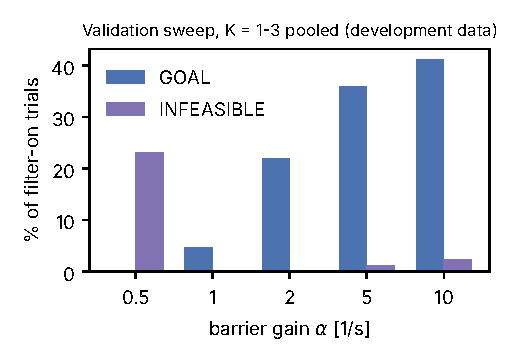
\includegraphics[width=0.9\columnwidth]{../figures/F1_validation_sweep.pdf}
\caption{Validation sweep (development data): filter-on GOAL and INFEASIBLE share per gain, $K=1$--3 pooled.}\label{fig:f1}
\end{figure}
\begin{figure*}[t]\centering
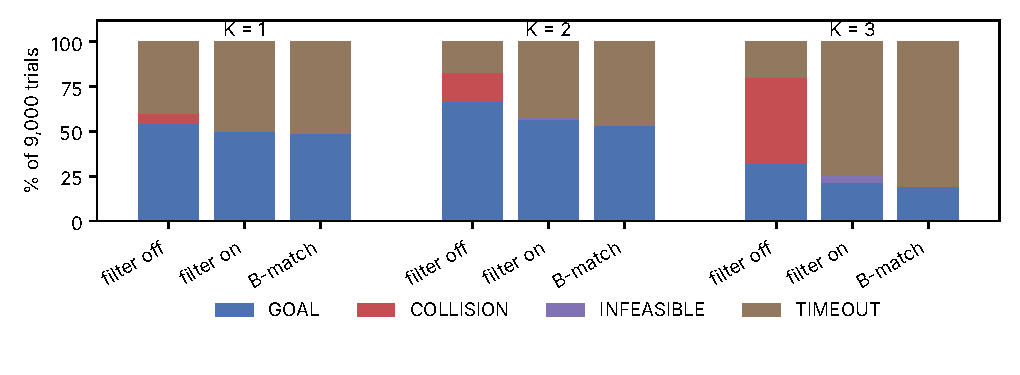
\includegraphics[width=0.8\textwidth]{../figures/F2_final_outcomes.pdf}
\caption{Final-test outcome shares per density for filter off, filter on ($\alpha^\star$) and B-match.}\label{fig:f2}
\end{figure*}
\begin{figure*}[t]\centering
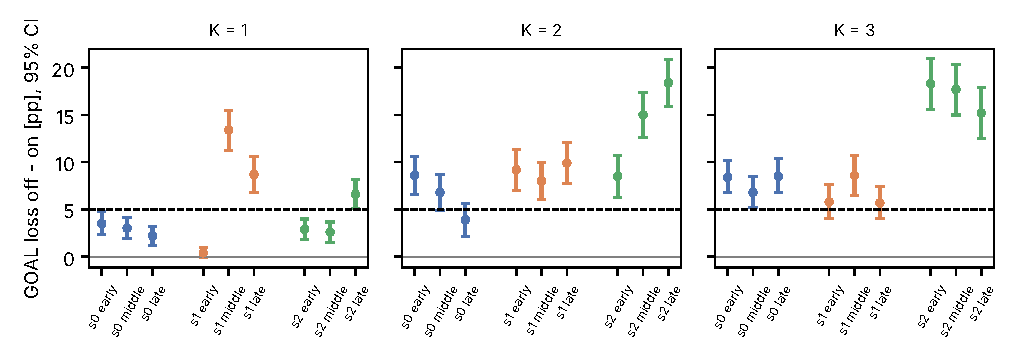
\includegraphics[width=0.85\textwidth]{../figures/F3_per_actor_goal_loss.pdf}
\caption{Per-actor GOAL loss (off minus on) with descriptive 95\% Newcombe intervals, grouped by
training seed; dashed line: the 5\,pp margin of the pooled criterion (b).}\label{fig:f3}
\end{figure*}

\section{Exploratory mechanism analysis (exploratory, post hoc)}\label{sec:mechanism}
\emph{Everything in this section is exploratory and post hoc: categories, thresholds, groups and the
example were chosen after the confirmatory results were known, the analyses read only saved logs,
and they support no causal or confirmatory claim.}

\paragraph{Definitions.} TIMEOUTs are classified from the saved logs in this order, over the last 50
executed periods (the window): \emph{slow progress} (stalled flag off: the centroid-to-goal distance fell
by at least 0.05\,m over the window); \emph{intervention-active stall} (stalled, and the clipped nominal command
violated an enabled barrier row in at least half of the window; split by obstacle and neighbour rows);
\emph{near-goal parking stall} (stalled, not the previous class, final centroid within 0.30\,m of the
goal); \emph{other stall}. The repository files call the second class ``filter-induced stall''; the
name used here records only that the filter was overriding the command, not that it caused the stall.
Throughout, ``stall'' means little terminal progress toward the goal, not that the robots stopped; the
classes are operational labels, not identified causes.
``Reached goal region'' uses the minimum centroid distance over the trial, the parking class the final
one.

\paragraph{Stall classes.} Of \TOonTotal{} filter-on TIMEOUTs, \TOfi{} (\TOfiPct\%) were
intervention-active stalls, \TOfiObst{} of them involving obstacle rows; on the same layouts the
unfiltered run collided in \TOfiOffColl{} cases, where a stall replaced a collision, and reached GOAL in
\TOfiOffGoal. Another \TOng{} (\TOngPct\%) were near-goal parking stalls, \TOngOffTO{} of them on layouts
where the unfiltered run also timed out; \TOother{} were other stalls and \TOslow{} slow progress.

\paragraph{Lost and gained completions.} Per pair, a completion is \emph{lost} when the unfiltered run
reached GOAL and the filtered run did not, and \emph{gained} in the reverse case
(Table~\ref{tab:lostgained}, Fig.~\ref{fig:f7}; all 16 off-by-on outcome transition counts per density
are in \url{results/paper_revision/transitions_4x4.csv}). Pooled over $K=1$--3, \LostTotalAll{}
completions were lost and \GainTotalAll{} gained, a net GOAL loss of \NetLossAll{} pairs; at each
density the net loss divided by the number of pairs equals the criterion (b) estimate. Of the lost
completions, \LostFIAll{} ended in an intervention-active stall, \LostOtherTOAll{} in another TIMEOUT class
(\LostNgAll{} of them near-goal parking stalls), \LostInfAll{} as INFEASIBLE and \LostCollAll{} as
COLLISION. The gained completions were unfiltered COLLISION (\GainCollAll) and TIMEOUT (\GainTOAll)
runs; \GainInfAll{} came from INFEASIBLE, which the unfiltered arm never produced.

In \LostRgrNoAll{} of the \LostTotalAll{} lost pairs (\LostRgrNoPctAll\%; \LostRgrNoPctone\%,
\LostRgrNoPcttwo\% and \LostRgrNoPctthree\% at $K=1,2,3$) the filtered run never brought its
centroid within 0.30\,m of the goal before any failure; in \LostRgrYesAll{} (\LostRgrYesPctAll\%) it
did. An earlier version of this draft inferred from the marginal reached-goal-region rates that the
lost completions were mostly runs that never approached the goal; marginal rates cannot identify
the pairs involved, and this paired count replaces that inference. It aggregates the saved
reached-goal-region flags. Entering the goal region does not by itself establish a parking stall,
and the TIMEOUT classes are exploratory labels assigned from saved logs, not identified causes.

\begin{table*}[t]
\centering\footnotesize
\caption{Lost and gained completions, filter off $\to$ filter on (exploratory, post hoc), in pairs
out of \PairsPerDensity{} per density. Lost: off GOAL and on not GOAL, split by the filter-on outcome
(TIMEOUT classes as in the stall-class paragraph); gained: off not GOAL and on GOAL, split by the
filter-off outcome. Net GOAL loss = lost $-$ gained = off GOAL count $-$ on GOAL count. Last rows:
whether the filtered run of a lost pair reached the goal region (saved flag).}
\label{tab:lostgained}
\begin{tabular}{lcccc}
\toprule
 & $K=1$ & $K=2$ & $K=3$ & $K=1$--3\\
\midrule
Lost: intervention-active stall & \LostFIone & \LostFItwo & \LostFIthree & \LostFIAll\\
\quad other TIMEOUT class & \LostOtherTOone & \LostOtherTOtwo & \LostOtherTOthree & \LostOtherTOAll\\
\quad INFEASIBLE & \LostInfone & \LostInftwo & \LostInfthree & \LostInfAll\\
\quad COLLISION & \LostCollone & \LostColltwo & \LostCollthree & \LostCollAll\\
\quad total (\% of pairs) & \LostTotalone{} (\LostTotalPctone) & \LostTotaltwo{} (\LostTotalPcttwo) & \LostTotalthree{} (\LostTotalPctthree) & \LostTotalAll{} (\LostTotalPctAll)\\
\midrule
Gained: from COLLISION & \GainCollone & \GainColltwo & \GainCollthree & \GainCollAll\\
\quad from TIMEOUT & \GainTOone & \GainTOtwo & \GainTOthree & \GainTOAll\\
\quad from INFEASIBLE & \GainInfone & \GainInftwo & \GainInfthree & \GainInfAll\\
\quad total (\% of pairs) & \GainTotalone{} (\GainTotalPctone) & \GainTotaltwo{} (\GainTotalPcttwo) & \GainTotalthree{} (\GainTotalPctthree) & \GainTotalAll{} (\GainTotalPctAll)\\
\midrule
Net GOAL loss off$-$on, pairs (pp) & \NetLossone{} (\NetLossPctone) & \NetLosstwo{} (\NetLossPcttwo) & \NetLossthree{} (\NetLossPctthree) & \NetLossAll{} (\NetLossPctAll)\\
\midrule
Lost, filtered run reached goal region: & & & & \\
\quad no (\% of lost) & \LostRgrNoone{} (\LostRgrNoPctone) & \LostRgrNotwo{} (\LostRgrNoPcttwo) & \LostRgrNothree{} (\LostRgrNoPctthree) & \LostRgrNoAll{} (\LostRgrNoPctAll)\\
\quad yes (\% of lost) & \LostRgrYesone{} (\LostRgrYesPctone) & \LostRgrYestwo{} (\LostRgrYesPcttwo) & \LostRgrYesthree{} (\LostRgrYesPctthree) & \LostRgrYesAll{} (\LostRgrYesPctAll)\\
\bottomrule
\end{tabular}
\end{table*}
\begin{figure*}[t]\centering
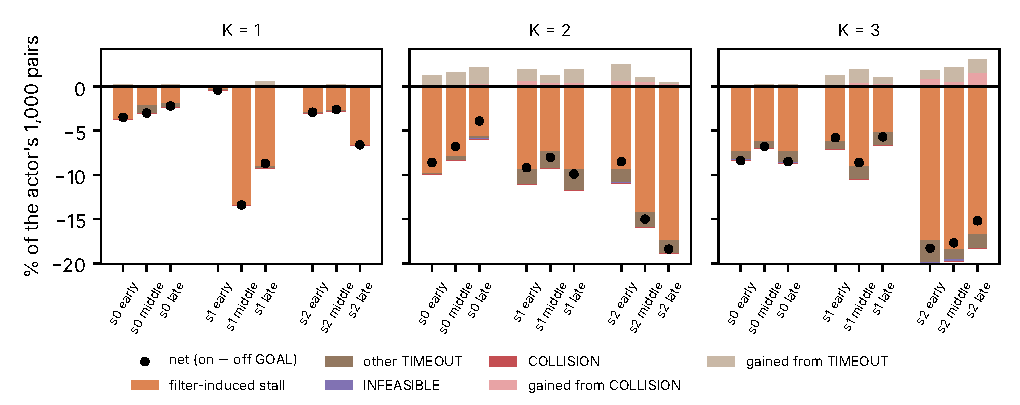
\includegraphics[width=0.85\textwidth]{../figures/F7_lost_gained.pdf}
\caption{Lost and gained completions per actor (exploratory, post hoc), as \% of each actor's 1{,}000
pairs, grouped by training seed. Below zero: lost completions stacked by filter-on outcome; above zero:
gained completions stacked by filter-off outcome. The dot is gained minus lost, the signed change in
GOAL (on minus off); Table~\ref{tab:lostgained} reports the net GOAL loss with the opposite sign (off
minus on). No lost completion ended in COLLISION (\LostCollAll{} pairs).}\label{fig:f7}
\end{figure*}

\paragraph{Groups A and B.} Group A (\GroupA{} pairs: unfiltered GOAL, filtered
intervention-active stall; \GroupAobst{} obstacle-labelled, \GroupAnb{} neighbour-only) and group B (\GroupB{} pairs:
both GOAL) were selected by observed outcome. The unfiltered runs of group A came closer to
obstacles (median sampled minimum surface clearance \GapAmedCm\,cm, group A only) than those of
group B (\GapBmedCm\,cm; Fig.~\ref{fig:f4}). Their applied commands violated at least one filter
obstacle row in \ACobstViolPct\% (A) versus \BCobstViolPct\% (B) of runs, and a robot-pair row in
\ACrrViolPct\% versus \BCrrViolPct\%.

\paragraph{Example (exploratory, post hoc).} Fig.~\ref{fig:f6} shows one group-A pair, chosen by a
rule fixed before plotting: the pair whose unfiltered minimum sampled obstacle clearance is closest to
the unrounded group-A median (\ExMedCm\,cm), ties by actor index, density and trial. In exact decimal
comparison \ExNtied{} candidates were equally close; the actor-index tie-break selected actor \ExActor,
$K=\ExK$, trial \ExTrial{} (clearance \ExGapCm\,cm). The unfiltered run reached GOAL
after \ExOffT{} periods with its closest approach at period \ExCaState; the filtered run's centroid
stalled from period \ExStallState. At that instant, robot \ExRobot{} (the robot with the smallest
obstacle cover barrier, $h=\ExCoverH$\,m$^2$, body clearance \ExCoverGapCm\,cm) is shown with its
cover disc. This is a geometric selection: it does not show that this robot or constraint caused the
stall, and a centroid stall does not mean that every robot stopped.

\paragraph{Clearance thresholds.} Of all trials, \ThrOffGoal\% reached GOAL unfiltered, and
\ThrMatchObstFive\% did so while keeping a sampled minimum obstacle clearance of at least 5\,cm (a
post hoc cut equal to $\ell$; Fig.~\ref{fig:f5} shows all thresholds),
against a filter-on GOAL rate of \ThrOnGoal\% on the same layouts (Fig.~\ref{fig:f5}). This
describes how close the unfiltered runs came to obstacles; it does not measure what a buffer or
any filter would cost. Among unfiltered GOAL trials the descriptive AUC of the unfiltered minimum
obstacle clearance for ``filtered run did not reach GOAL'' was \AucPooled; it is in-sample, post hoc
and partly mechanical, because obstacle rows activate at small clearance, and is not a validated
predictor.

\paragraph{Infeasibility.} All \InfTotal{} INFEASIBLE trials were reproduced (\InfRepro{} of
\InfTotal) by the unchanged filter code at the saved states in an earlier audit. An infeasible QP
has no optimal active set, so the audit recorded, for each infeasible robot, the zero-command slack of
every enabled row (the normalised value $(g^\top u-b)/\|g\|$ at $u=0$, negative when the row is
violated) and examined the row with the most negative slack. In every case that row's barrier value was
within \InfHdiffMax{}\,m$^2$ of its stand-off $h^\star$ (Section~\ref{sec:system}), with slack between
\InfSlackMin{} and \InfSlackMax. The zero command violated between \InfRowsMin{} and \InfRowsMax{}
enabled rows (two or more for \InfRowsTwoPlus{} of \InfRobots{} robots), and recomputing the binding
slack in float32 changed its sign for \InfFlipFthirtytwo{} of them. \InfNear{} of \InfRobots{} met a
near-boundary diagnostic fixed before the (post hoc) audit computation ($|\text{slack}|\le10^{-6}$ and
$|h-h^\star|\le10^{-3}$\,m$^2$). The infeasible states thus sat where stopping is only marginally
inadmissible, and the evaluation of that row is sensitive to rounding. This does not show that the full
QP would become feasible, that the zero command would satisfy every other row, or that the trial would
end differently: the audit did not identify which rows and box limits jointly conflicted, and the effect
on whole-QP feasibility and on subsequent outcomes is unresolved. The stand-off exists
at every gain, and the development sweep had INFEASIBLE outcomes at every gain, most at $\alpha=0.5$
(\SelInfhalf), so these events are not specific to $\alpha\Delta=1$.

\paragraph{Transit.} Writing $n=(p_i-p_j)/d$, the pair row bounds robot $i$'s closing speed
$-n^\top\dot p_i$ by $\alpha(h_{ij}-h^\star_{ij})/(4d)$, with $h^\star_{ij}=\delta_{ij}(d)/\alpha$. During
formation transit (centroid more than 0.30\,m from the goal) this cap had median
\CapMedMin--\CapMedMax\,m/s, above the largest barrier-point speed $V_p\approx\Vp$\,m/s, and was binding
in \CapBindMin--\CapBindMax\% of the periods in which a moving robot closed on a neighbour, so neighbour
rows seldom limited transit.

\begin{figure*}[t]\centering
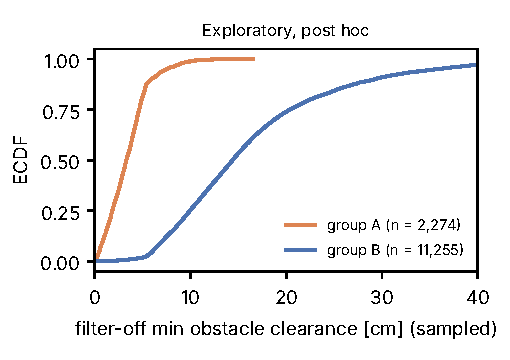
\includegraphics[width=0.42\textwidth]{../figures/F4_clearance_groups.pdf}\hspace{0.04\textwidth}
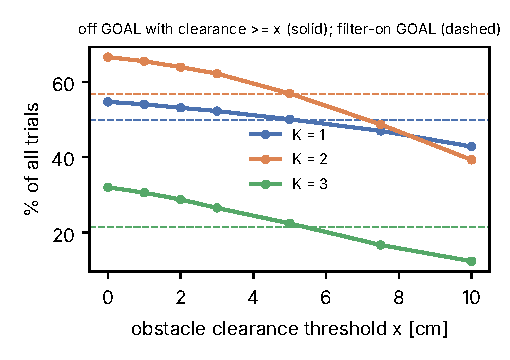
\includegraphics[width=0.42\textwidth]{../figures/F5_matched_denominator.pdf}
\caption{Exploratory, post hoc. Left: unfiltered minimum obstacle clearance (sampled), group A
vs group B. Right: share of all trials that reached GOAL unfiltered with clearance at least
$x$, per density, with the filter-on GOAL rate (dashed).}\label{fig:f4}\label{fig:f5}
\end{figure*}
\begin{figure*}[t]\centering
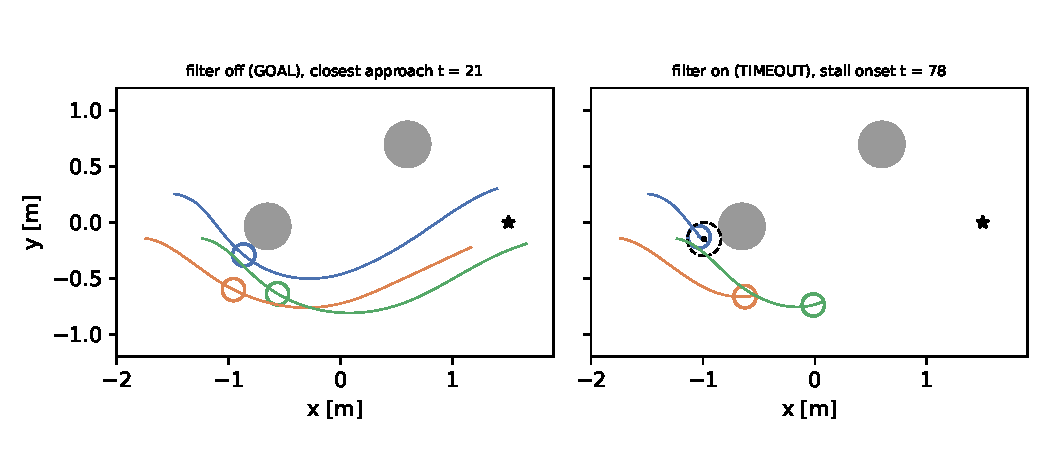
\includegraphics[width=0.8\textwidth]{../figures/F6_example_trajectory.pdf}
\caption{Exploratory, post hoc example. Selection rule (fixed before plotting): among group-A pairs, the pair
whose filter-off minimum sampled obstacle clearance is closest to the unrounded group-A median; ties by actor
index, density, then trial. Left: filter off, bodies at the closest-approach instant. Right: filter on,
bodies at stall onset (first state from which the centroid stays within 0.05\,m of its final position), with
the cover disc (dashed, radius $R+\ell$) of the robot with the smallest obstacle barrier at that instant (ties by
robot index). Star: goal. Geometric selection only; not evidence of cause.}\label{fig:f6}
\end{figure*}

\section{Discussion}\label{sec:discussion}
\paragraph{Hypotheses and evidence.}
\emph{H1 (collisions fall).} Descriptively consistent for these actors: with the filter on there were
\CollOnone, \CollOntwo{} and \CollOnthree{} collisions against \CollOffone, \CollOfftwo{} and
\CollOffthree{} with the filter off. Zero filter-on collisions is consistent with the conditional guarantee
of Section~\ref{sec:system} and is numerical evidence on the evaluated trajectories; it does not certify
the solver, verify every assumption or establish floating-point safety; the \InfOnone, \InfOntwo{} and \InfOnthree{} trials whose QP became
infeasible ended without a fallback, so their later course is unknown, and the uncertified B-match also
had no collisions. The confirmatory endpoint is the composite
COLLISION-or-INFEASIBLE, whose reduction met criterion (a) at every density (Table~\ref{tab:conf});
collision counts alone were not a confirmatory endpoint.
\emph{H2 (formation error and completion time rise, more so in denser layouts).} The common-prefix
formation increase was \Cincone, \Cinctwo{} and \Cincthree\,m at $K=1,2,3$. These point estimates
exceed the 0.01\,m margin, and criterion (c), which tests non-inferiority, was not met at any
density: non-inferiority was not established (confirmatory). This is not the same as a confirmatory
test showing that the increase exceeds the margin. The estimates increase with
density, but no density trend was tested, so the ``more so in denser layouts'' part is not
established; here density changes both the obstacle count and the distance from the final training
mixture ($K=2,5,8$), so trends across $K$ would not be effects of clutter alone. In pairs where both arms
reached GOAL the full-trajectory formation error rose by only \BothGoalFormone, \BothGoalFormtwo{} and
\BothGoalFormthree\,m (pre-declared secondary, conditioned on joint success), so most of the
common-prefix increase arises in pairs whose trajectories diverged. GOAL rates were lower with the
filter at every density (descriptive 95\% intervals for the loss exclude zero); criterion (b) tests
non-inferiority and was not met, and GOAL rate is not the completion-time part of H2. In joint-success
pairs the time to goal changed little (equal-actor mean \TtgEqOnone, \TtgEqOntwo{} and \TtgEqOnthree{} periods;
Table~\ref{tab:ttg}), and this conditional analysis does not estimate the completion-time cost.
\emph{H3 (failures under filtering come from deadlock or infeasible steps rather than slower
progress).} Of the \HthreeNongoalAll{} filter-on trials that did not reach GOAL, \HthreeShareAll\%
ended INFEASIBLE or as TIMEOUT with the protocol's stalled flag, and \HthreeMovingAll{} were TIMEOUTs
still closing on the goal at the horizon (stalled flag pre-declared as secondary, descriptive). The flag,
however, accompanied \OffStallOfTOone, \OffStallOfTOtwo{} and \OffStallOfTOthree\% of TIMEOUTs with the
filter off as well (\OnStallOfTOone, \OnStallOfTOtwo{} and \OnStallOfTOthree\% with it on): at this
horizon almost every TIMEOUT ends with little progress toward the goal in its last 50 periods. The flag
describes that low terminal progress; it cannot distinguish a team parked near the goal from one held
by obstacles or by the filter, and its high prevalence in both arms does not identify filter-specific
deadlock, so it does not test H3. In the exploratory classes of Section~\ref{sec:mechanism}, \TOfiPct\% of
filter-on TIMEOUTs were intervention-active stalls and \TOngPct\% near-goal parking stalls, \TOngOffTO{}
of the latter on layouts where the unfiltered run also timed out.

\paragraph{Collisions versus stalls.} With the filter on there were no collisions (\CollOnone,
\CollOntwo{} and \CollOnthree{} at $K=1,2,3$; the remaining failures were INFEASIBLE;
Table~\ref{tab:conf}); in the exploratory classification most filtered timeouts were
intervention-active stalls, mostly on layouts where the unfiltered run collided or reached GOAL. We read
this as a description of where the lost completions occurred, not as a causal attribution; stalls of
this kind may reflect the undesirable equilibria that CBF-QP filters can introduce \cite{reis2021}, which
these logs do not establish. The completions lost in group A involved unfiltered runs that passed close to obstacles
(median \GapAmedCm\,cm, group A only; Fig.~\ref{fig:f4}), inside the \CoverBandLoCm--\CoverBandHiCm\,cm
clearance band a stopped robot needs (Section~\ref{sec:system}), although the actors were trained with a
proximity penalty below 15\,cm. These lost completions are where the policy's habitual clearance and the
filter's conservatism (cover disc and margin) conflict; which side to change is not identified here.
The filter reached GOAL \OnBmGoalMin--\OnBmGoalMax{} percentage points more often than B-match on the
same layouts, with more INFEASIBLE outcomes (B-match cannot be infeasible by construction).

\paragraph{Gain at the lemma boundary.} The selected gain gives $\alpha^\star\Delta=1$, the largest gain
Lemma~1 admits. The lemma still keeps $h\ge0$ over each period, though with no strictly positive
endpoint bound from the initial barrier alone. The infeasible states sat at the stand-off, which exists
at every gain, and infeasibility occurred at every gain in the development sweep, so we do not attribute
it to $\alpha^\star\Delta=1$ alone; a numerical contribution of the boundary gain is not excluded.

\paragraph{Predictions and an unaddressed recommendation.} The locked protocol contains an analytic
prediction: at $\alpha=0.5$ the zero command becomes admissible for a robot pair only at a barrier-point
separation of 0.668\,m, above the nominal 0.520\,m spacing, so $\alpha=0.5$ was expected to conflict
strongly with holding the formation. A methodology report written before the validation sweep, but
committed only after the final test (\texttt{docs/methodology/README.md}), also predicted that the
selected gain would lie in $[5,10]$. The sweep selected $\alpha^\star=\AlphaStar$, the largest admissible
grid value, and gave \SelGoalhalf{} filter-on GOAL outcomes with \SelInfhalf{} INFEASIBLE at
$\alpha=0.5$ (Fig.~\ref{fig:f1}); this concerns feasibility and completion, not a measured formation
conflict. The same report estimated the implemented obstacle margin at about \MarginRatioObst{} times a
tight one-sided margin at $d=D_o$, predicted that the cover-disc barrier would cost completions, and
recommended advisor review of the margin; the margin was locked unchanged without that review. How much
of the GOAL loss is due to margin conservatism, cover-disc geometry or the equal split was not tested.

\paragraph{Remark (zero-command-admissible rows).} For these offset-point barriers the second-order
margin can be evaluated at the held command instead of bounded over the input set: $\delta$ is replaced
by a term proportional to $|\omega|$, written as two affine rows per barrier, which makes the zero
command admissible whenever $h\ge0$ in exact arithmetic (\texttt{docs/CBF\_DESIGN.md}). Its ingredients
are existing ideas \cite{breeden2022,vandenberg2011,chen2021}. It would move the marginal state from the
stand-off to $h=0$ but not remove sensitivity to rounding, and it was not implemented or evaluated here.

\paragraph{Practical implications (suggestions, each tied to a result; not findings).}
(i) Pair the filter with an infeasibility fallback and a deadlock-recovery rule: with neither,
\LostFIAll{} of the \LostTotalAll{} lost completions ended in intervention-active stalls and \InfTotal{}
trials ended INFEASIBLE. This study does not evaluate either remedy.
(ii) Treat the stand-off with an explicit tolerance rule or zero-command-admissible rows, in a
separately designed follow-up (infeasibility audit). In the development sweep GOAL increased across the
gain grid, while infeasibility was non-monotonic: lowering $\alpha$ from 10 to 5 reduced both GOAL
(\SelGoalten{} to \SelGoalfive) and INFEASIBLE outcomes (\SelInften{} to \SelInffive; Fig.~\ref{fig:f1}).
These validation results do not show that a lower gain would improve overall usefulness.
(iii) In this post hoc analysis lost completions coincided with small unfiltered clearances on the same
layouts (AUC \AucPooled, in-sample and partly mechanical); whether a clearance statistic from
independent rollouts predicts a policy's filter cost was not tested.
(iv) Include a brake baseline on the same rows: here B-match, which cannot be infeasible by construction
and carries no safety certificate, had no collisions and reached GOAL
\OnBmGoalMin--\OnBmGoalMax{} percentage points less often than the filter (descriptive, this scenario).
(v) Where a policy habitually passes inside the clearance band a stopped robot needs, the cost may be
reduced from either side (less conservative barrier geometry or margin, or training that keeps more
clearance); the proximity penalty used here did not keep the group-A passes outside that band.

\section{Limitations}
The study uses one simulated scenario, one filter instantiation (cover disc with $\ell=5$\,cm,
two-sided state-only margins, equal split, the largest admissible gain, no fallback) and nine actors from
three training runs of one custom MAPPO implementation. The actors did not meet the study's filter-off
competence gate, which was pooled over $K=2,5,8$; the primary densities $K=1,2,3$ were chosen after
their filter-off validation results had been seen; and $K=1$ and $K=3$ are absent from the final
curriculum stage, though encountered in earlier stages. All intervals reflect layout sampling
for fixed actors, not variation across training runs. The margins are the author's judgement.
Validation layouts controlled curriculum advancement and were reused for gain tuning. The formation
criterion covers the common executed prefix only. Time to goal is analysed only in joint-success pairs.
The safety guarantee is analytic but conditional on A1--A9; A1 holds in simulation only to float32
accuracy, which the zero-collision count checks numerically. The exploratory analyses are selected by
observed outcome and descriptive.
Three related-work classifications rest on abstracts only (Table~\ref{tab:related}).

\section{Future work}
Sensing noise or delay would test whether the unfiltered small-clearance passes stay collision-free.
An infeasibility fallback and deadlock recovery, zero-command-admissible rows or an explicit tolerance
rule at the stand-off, less conservative barrier geometry, and clearance-aware or filter-aware
retraining are candidate follow-ups, as is a policy family that passes the competence gate. Any such study would use the reserved, unused
5{,}000{,}000--5{,}999{,}999 layout block under its own locked protocol and disclose which of the
present post-test findings informed it.

\section{Reproducibility}
{\sloppy Code, configuration, saved logs and analyses are in \url{https://github.com/mahdisallam860/cbf-marl-filter-study}
(branch \texttt{claude/elegant-hopper-v8jxlv}). Protocol lock: commit \texttt{9baf6d7}; selected gain:
\texttt{4fffe62}; final test: \texttt{e23f8c3} (per-step logs \texttt{41ae3d4}); mechanism analyses:
\texttt{df78812}, \texttt{c2e331a}. Layout seeds: validation $2{,}000{,}000+K$; final test
$4{,}000{,}000+1{,}000p+K$ for actor index $p$; the block $5{,}000{,}000$--$5{,}999{,}999$ is reserved and
unused. The per-step logs of every final-test trial (poses, raw, clipped and applied commands,
interventions, brake activations) are committed, so all analyses here can be repeated without
re-running trials.\par}

\section{Mandatory disclosures}\label{sec:disclosures}
\begin{itemize}
\item The margins and protocol decisions were chosen by the author without advisor review; advisor agreement has not been obtained.
\item The protocol was locked before any filter-on data with the frozen MAPPO actors existed, but after engineering stress tests with random and adversarial stand-in controllers and demonstration runs with an obstacle-blind stand-in controller (the locked document's wording ``before any filter-on data existed'' is corrected here).
\item Filter-off validation results had been seen before the protocol was locked.
\item The checkpoint rule was committed before the checkpoints were evaluated, but after earlier validation results were seen.
\item The validation layouts controlled curriculum stage advancement and were reused as development data for gain tuning.
\item The primary densities $K=1,2,3$ were chosen after the filter-off gate had failed and the actors' filter-off validation results had been seen.
\item The methodology report was committed after the final test.
\item The mechanism categories were chosen after the confirmatory results were known.
\item The post-test decision rule was not committed before the mechanism results were read.
\item The locked protocol labels the paired interval for criteria (a) and (b) ``Newcombe method~10'' but describes it as uncorrected (``without continuity correction''), which is method~8; the analysis code implements the description. With method~10 every bound changes by less than 0.001 percentage points and no criterion changes (found after the final test). The filter-on versus B-match intervals in Table~\ref{tab:onbm}, computed after this was found, use method~10 itself.
\item The example in Fig.~\ref{fig:f6} was first recorded as the unique nearest candidate; exact decimal comparison shows two equally close candidates, and the stated actor-index tie-break selects the same pair (regenerated metadata in \url{results/paper_revision/example_selection.json}).
\item One of the \TrialsTotal{} final-test trials (s2\_early, $K=3$, trial 646) started with a negative obstacle cover barrier ($h=\AfiveH$\,m$^2$, body clearance \AfiveGap\,m), an exception to assumption A5; it is kept in all confirmatory numbers.
\item Training seed~1 crashed at iteration 565 and was resumed from its saved iteration-546 state without restoring the environments or the global random-number state; iterations 547--565 were discarded. Actors s1\_middle and s1\_late come from the resumed run (Section~\ref{sec:policy}).
\item Claims cover these nine fixed actors in this simulated scenario only.
\item The safety guarantee of Section~\ref{sec:system} is conditional on A1--A9; A1 holds in simulation only to float32 accuracy.
\item The near-boundary diagnostic in Section~\ref{sec:mechanism} was fixed before the post hoc audit computation, not in the locked protocol.
\item The MAPPO implementation is custom and was sanity-checked only on the stock VMAS navigation task.
\end{itemize}

\section{Conclusion}
Under the pre-set criteria, this execution-time CBF-QP filter (cover disc, two-sided state-only
margins, $\alpha^\star\Delta=1$, no fallback) was not shown useful for these nine frozen MAPPO actors at
any of the three densities: it reduced collision-or-infeasible outcomes but did not establish
non-inferiority in goal completion or common-prefix formation error. At $K=1$ the GOAL-loss estimate lay
inside its margin and the shortfall was concentrated in one training run; at $K=2,3$ both estimates
exceeded their margins. A brake on the same rows had no collisions and reached GOAL slightly less often.
The actors had not met the study's competence gate (pooled over $K=2,5,8$), so the filter's cost on
policies that keep more clearance is not known.

\section*{Acknowledgment}
The code, analyses and this draft were produced with
substantial assistance from an AI coding assistant (Claude, Anthropic) under the author's direction.
Every number in the text is generated by committed scripts from committed result files
(\texttt{scripts/paper\_numbers.py}, \texttt{paper/numbers.tex}). The author is responsible for the content.

\begin{thebibliography}{99}
\bibitem{brunke2022} L.~Brunke, M.~Greeff, A.~W.~Hall, Z.~Yuan, S.~Zhou, J.~Panerati, A.~P.~Schoellig, ``Safe learning in robotics: From learning-based control to safe reinforcement learning,'' \emph{Annual Review of Control, Robotics, and Autonomous Systems}, vol.~5, pp.~411--444, 2022, doi:10.1146/annurev-control-042920-020211.
\bibitem{ames2019} A.~D.~Ames, S.~Coogan, M.~Egerstedt, G.~Notomista, K.~Sreenath, P.~Tabuada, ``Control barrier functions: Theory and applications,'' Proc. 18th European Control Conference (ECC), 2019, pp.~3420--3431, doi:10.23919/ECC.2019.8796030.
\bibitem{wang2017} L.~Wang, A.~D.~Ames, M.~Egerstedt, ``Safety barrier certificates for collisions-free multirobot systems,'' \emph{IEEE Transactions on Robotics}, vol.~33, no.~3, pp.~661--674, 2017, doi:10.1109/TRO.2017.2659727.
\bibitem{deng2026} Z.~Deng, Q.~Li, M.~Zhang, W.~Chen, ``Safe multi-agent reinforcement learning through neural graph control barrier functions,'' Proc. AAMAS 2026, pp.~3232--3234, extended abstract, doi:10.65109/KRTJ4225.
\bibitem{dawood2025} M.~Dawood, S.~Pan, N.~Dengler, S.~Zhou, A.~P.~Schoellig, M.~Bennewitz, ``Safe multi-agent reinforcement learning for behavior-based cooperative navigation,'' \emph{IEEE Robotics and Automation Letters}, vol.~10, no.~6, pp.~6256--6263, 2025, doi:10.1109/LRA.2025.3560830.
\bibitem{cai2021} Z.~Cai, H.~Cao, W.~Lu, L.~Zhang, H.~Xiong, ``Safe multi-agent reinforcement learning through decentralized multiple control barrier functions,'' arXiv:2103.12553, 2021.
\bibitem{qin2021} Z.~Qin, K.~Zhang, Y.~Chen, J.~Chen, C.~Fan, ``Learning safe multi-agent control with decentralized neural barrier certificates,'' ICLR 2021, arXiv:2101.05436.
\bibitem{zhang2025dgppo} S.~Zhang, O.~So, M.~Black, C.~Fan, ``Discrete GCBF proximal policy optimization for multi-agent safe optimal control,'' ICLR 2025, arXiv:2502.03640.
\bibitem{choi2025} J.~J.~Choi, J.~J.~Aloor, J.~Li, M.~G.~Mendoza, H.~Balakrishnan, C.~Tomlin, ``Resolving conflicting constraints in multi-agent reinforcement learning with layered safety,'' Robotics: Science and Systems (RSS), 2025, doi:10.15607/RSS.2025.XXI.094.
\bibitem{zhang2025gcbf} S.~Zhang, O.~So, K.~Garg, C.~Fan, ``GCBF+: A neural graph control barrier function framework for distributed safe multiagent control,'' \emph{IEEE Transactions on Robotics}, vol.~41, pp.~1533--1552, 2025, doi:10.1109/TRO.2025.3530348.
\bibitem{agarwal2021} R.~Agarwal, M.~Schwarzer, P.~S.~Castro, A.~Courville, M.~G.~Bellemare, ``Deep reinforcement learning at the edge of the statistical precipice,'' NeurIPS 2021, vol.~34, pp.~29304--29320, arXiv:2108.13264.
\bibitem{vinod2022} A.~P.~Vinod, S.~Safaoui, A.~Chakrabarty, R.~Quirynen, N.~Yoshikawa, S.~Di~Cairano, ``Safe multi-agent motion planning via filtered reinforcement learning,'' IEEE International Conference on Robotics and Automation (ICRA), 2022 (MERL TR2022-053). \url{https://www.merl.com/publications/docs/TR2022-053.pdf}
\bibitem{singletary2020} A.~Singletary, Y.~Chen, A.~D.~Ames, ``Control barrier functions for sampled-data systems with input delays,'' IEEE Conference on Decision and Control (CDC), 2020; arXiv:2005.06418.
\bibitem{breeden2022} J.~Breeden, K.~Garg, D.~Panagou, ``Control barrier functions in sampled-data systems,'' \emph{IEEE Control Systems Letters}, vol.~6, pp.~367--372, 2022, doi:10.1109/LCSYS.2021.3076127. \url{https://arxiv.org/abs/2103.03677} (Theorem~3, second-order approach; checked against arXiv v2 on 2026-10-26; the paper uses the opposite sign convention for $h$)
\bibitem{tan_zocbf} X.~Tan, E.~Da\c{s}, A.~D.~Ames, J.~W.~Burdick, ``Zero-order control barrier functions for sampled-data systems with state and input dependent safety constraints,'' arXiv:2411.17079, 2024.
\bibitem{liu_sacbf} S.~Liu, W.~Xiao, C.~A.~Belta, ``Sampling-aware control barrier functions for safety-critical and finite-time constrained control,'' arXiv:2511.11897, 2025.
\bibitem{vandenberg2011} J.~van~den~Berg, S.~J.~Guy, M.~Lin, D.~Manocha, ``Reciprocal n-body collision avoidance,'' in \emph{Robotics Research}, Springer Tracts in Advanced Robotics, vol.~70, Springer, 2011, doi:10.1007/978-3-642-19457-3\_1.
\bibitem{chen2021} Y.~Chen, A.~Singletary, A.~D.~Ames, ``Guaranteed obstacle avoidance for multi-robot operations with limited actuation: A control barrier function approach,'' \emph{IEEE Control Systems Letters}, vol.~5, no.~1, pp.~127--132, 2021.
\bibitem{emam2019} Y.~Emam, P.~Glotfelter, M.~Egerstedt, ``Robust barrier functions for a fully autonomous, remotely accessible swarm-robotics testbed,'' arXiv:1909.02966, 2019.
\bibitem{kim2026} T.~Kim, ``Is your safe controller actually safe? A critical review of CBF tautologies and hidden assumptions,'' arXiv:2603.06954, 2026.
\bibitem{yang2019} G.~Yang, C.~Belta, R.~Tron, ``Self-triggered control for safety critical systems using control barrier functions,'' arXiv:1903.03692, 2019.
\bibitem{yu2022mappo} C.~Yu, A.~Velu, E.~Vinitsky, J.~Gao, Y.~Wang, A.~Bayen, Y.~Wu, ``The surprising effectiveness of PPO in cooperative multi-agent games,'' NeurIPS Datasets and Benchmarks Track, 2022; arXiv:2103.01955.
\bibitem{bettini2022vmas} M.~Bettini, R.~Kortvelesy, J.~Blumenkamp, A.~Prorok, ``VMAS: A vectorized multi-agent simulator for collective robot learning,'' Proc. 16th International Symposium on Distributed Autonomous Robotic Systems (DARS), Springer, 2022.
\bibitem{reis2021} M.~F.~Reis, A.~P.~Aguiar, P.~Tabuada, ``Control barrier function-based quadratic programs introduce undesirable asymptotically stable equilibria,'' \emph{IEEE Control Systems Letters}, vol.~5, no.~2, 2021, doi:10.1109/LCSYS.2020.3004797; arXiv:2003.07819.
\bibitem{newcombe1998} R.~G.~Newcombe, ``Improved confidence intervals for the difference between binomial proportions based on paired data,'' \emph{Statistics in Medicine}, vol.~17, pp.~2635--2650, 1998.
\end{thebibliography}
\end{document}
